\section{Simulation}\insertloftspace
\setcounter{figure}{0}\setcounter{table}{0}

\hspace{\parindent} In parallel to the design, we simulated the operation of the robot using Matlab, Simulink and python. The work explained from now on is done on the last prototype presented in the previous section. However, the principle applied has been the same throughout the project. The simultaneous work was important in order to anticipate the delays due to the manufacturing of the robot. 

\subsection{Robot kinematics}

\textbf{Definition :} Given a vector $x=[x_1 x_2 x_3]^T \in \mathbb{R}^3$, we define : 
\begin{center}
    $[x] = \begin{bmatrix}
        0 & -x_3 & x_2 \\
        x_3 & 0 & -x_1 \\
        -x_2 & x_1 & 0 \\
    \end{bmatrix}$
\end{center}

\noindent\textbf{Definition :} Given two vectors $x$ and $y$ in $\mathbb{R}^3$, we define : $x\times y = [x]\cdot y$

\bigbreak
\noindent\textbf{Definition :} For a joint, we define the pitch $h = \frac{v}{w}$ with v : the linear speed and w the angular speed

\bigbreak
\noindent\textbf{Definition :} The screw is a $6\times1$ vector that represent the angular velocity when $\dot{\theta}=1$ and the linear velocity of the origin when $\dot{\theta}=1$. $S = \begin{bmatrix} s_w\\s_v\end{bmatrix}$ with $s_v = hw-s_w\times q$ where h is the pitch and q is a point on the 

\noindent\textbf{Definition :} For a given reference frame, a screw axis S is written as 
\begin{center}
    $S=\begin{bmatrix}
        s_w\\s_v
    \end{bmatrix}$
\end{center}
where either (i) $\|s_w\|$ = 1 or (ii) $\|s_w\|$ = 0 and $\|s_v\|$ = 1. If the pitch is finite ($h$ = 0 for a pure rotation), then $s_v = hs_w-s_w\times q$ where q is a point on the axis of the screw

\bigbreak
The figure below shows the kinematics schema of the robot. The figure defines an \{s\} frame at the bottom, an \{e\} frame at the end effector position and a \{c\} frame at the camera position. The robot is at is home configuration. The joint are represented with the rotation (positive rotation about the axes is by the right hand rule).

\bigbreak 
The parameters can be found with Onshape and are listed below: 

\begin{center}
    \fcolorbox{black}{white}{
        \begin{minipage}{0.8\linewidth}
            $L_0 = 0.069m$ \hspace{3cm} $d_0 = 0m$ \hfill $h_0 = 0.06m$ \\
            $L_1 = 0.116m$ \hspace{3cm} $d_1 = 0.018m$ \\ 
            $L_2 = 0.16m$ \hspace{3.2cm} $d_2 = 0.042m$ \\ 
            $L_3 = 0.155m$ \hspace{3cm} $d_3 = 0.01413m$ \\ 
            $L_c = 0.053m$ \hspace{3cm} $d_c = 0.0105m$ \hfill $h_c = 0.0815m$ \\
            $L_e = 0.2377m$ \hfill $d_e = 0.0105$ \hfill $h_e = 5.10^{-5}m$ \\
        \end{minipage}
    }
\end{center}

\begin{figure}[ht]
    \centering
    \includegraphics[width=0.8\textwidth]{images/Section04/kinematics\_schema.png}
    \caption{Kinematics schema}
    \label{fig:mesh10}
\end{figure}
\FloatBarrier

\bigbreak
We can then define $M_c$ and the $M_e$ the transformation matrix ($T_{sc}$ and $T_{se}$) when the robot is at its home configuration. 

\bigbreak
\begin{center}
    $
    M_c = \begin{bmatrix}
        0 & 0 & 1 & -h_0-L_3-h_c\\
        0 & -1 & 0 & d_1-d_2+d_3+d_c\\
        1 & 0 & 0 & l_0+l_1+l_2+l_c\\
        0 & 0 & 0 & 1
    \end{bmatrix}
    $
    and
    $
    M_e = \begin{bmatrix}
        0 & 0 & 1 & -h_0-L_3-h_c\\
        0 & -1 & 0 & d_1-d_2+d_3+d_c\\
        1 & 0 & 0 & l_0+l_1+l_2+l_c\\
        0 & 0 & 0 & 1
    \end{bmatrix}
    $
\end{center}

\subsubsection{Base frame}

\hspace{\parindent} In this subsection we study the kinematics parameters in the base frame \{s\}. It will be the one used in the followings sections.

\bigbreak
The rotation axis $S_{w_i}$ of each joint  in \{s\} are : 
\begin{center}
    $S_{w_1} = \begin{bmatrix} 0 \\ 0 \\ -1\end{bmatrix}$,
    $S_{w_2} = \begin{bmatrix} 0 \\ 1 \\ 0\end{bmatrix}$,
    $S_{w_3} = \begin{bmatrix} 0 \\ -1 \\ 0\end{bmatrix}$,
    $S_{w_4} = \begin{bmatrix} 0 \\ -1 \\ 0\end{bmatrix}$,
\end{center}

\bigbreak
We can also write the position of each joint  $q_1,q_2,q_3,q_4,q_c,q_e$ in \{s\}. Lining up the position as columns, we get : 

\begin{center}
    $
    \begin{bmatrix}
        -h_0 & -h_0 & -h_0 & -h_0-L_3 & -h_0-L_3-h_c & -h_0-L_3-L_e  \\
        0 & d_1 & d_1-d_2 & d_1-d_2+d_3 & d_1-d_2+d_3+d_c & d_1-d_2+d_3+d_e \\
        L_0 & L_0+L_1 & L_0+L_1+L_2 & L_0+L_1+L_2 & L_0+L_1+L_2+L_c & L_0+L_1+L_2+h_e \\
    \end{bmatrix}
    $
\end{center}

\bigbreak
There are all pure rotation joint, using the position, the rotation axis and the formula define in above we can calculate the screw axis $S_1,S_2,S_3,S_4$ in \{s\}.. Lining up them as columns, we get : 

\begin{center}
    $S_{list} = 
    \begin{bmatrix}
        0 & 0 & 0 & 0 \\
        0 & 1 & -1 & -1 \\
        -1 & 0 & 0 & 0 \\
        0 & -L_0-L_1 & L_0+L_1+L_2 & L_0+L_1+L_2 \\
        -h_0 & 0 & 0 & 0 \\
        0 & -h_0 & h_0 & h_0+L_3
    \end{bmatrix}
    $
\end{center}

\subsubsection{End effector frame}

\hspace{\parindent} In this subsection we study the kinematics parameters in the end effector frame \{e\}. However, it is not the one that will be use later. 

\bigbreak
The rotation axis $S_{w_i}$ of each joint  in \{e\} are : 
\begin{center}
    $S_{w_1} = \begin{bmatrix} -1 \\ 0 \\ 0\end{bmatrix}$,
    $S_{w_2} = \begin{bmatrix} 0 \\ -1 \\ 0\end{bmatrix}$,
    $S_{w_3} = \begin{bmatrix} 0 \\ 1 \\ 0\end{bmatrix}$,
    $S_{w_4} = \begin{bmatrix} 0 \\ 1 \\ 0\end{bmatrix}$,
\end{center}

\bigbreak
We can also write the position of each joint  $q_1,q_2,q_3,q_4,q_c,q_e$ in \{e\}. Lining up the position as columns, we get : 

\begin{center}
    $
    \begin{bmatrix}
        -h_e-L_2-L_1 & -h_e-L_2 & -h_e & -h_e & -h_e+L_c & 0  \\
        d_e+d_3-d_2+d_1 & d_e+d_3-d_2 & d_e+d_3 & d_e & d_e-d_c & 0 \\
        L_e+L_3 & L_e+L_3 & L_e+L_3 & L_e & L_e-h_c & 0 \\
    \end{bmatrix}
    $
\end{center}

\bigbreak
There are all pure rotation joint, using the position, the rotation axis and the formula define in above we can calculate the screw axis $B_1,B_2,B_3,B_4$ in \{e\}.. Lining up them as columns, we get : 

\begin{center}
    $B_{list} = 
    \begin{bmatrix}
        -1 & 0 & 0 & 0 \\
        0 & -1 & 1 & 1 \\
        -1 & 0 & 0 & 0 \\
        0 & L_e+L_3 & -L_e-L_3 & -L_e \\
        -L_e-L_3 & 0 & 0 & 0 \\
        d_e+d_3-d_2+d_1 & h_e+L_2 & -h_e & -h_e
    \end{bmatrix}
    $
\end{center}

\subsection{URDF Format}

\hspace{\parindent} The Universal Robot Description Format (URDF) is an XML (eXtensible Markup Language) file format used by the Robot Operating System (ROS) to describe the kinematics, inertial properties, and link geometry of robots. A URDF file describes the joints and links of a robot:

\begin{itemize}
    \item \textbf{Joints :} Joints connect two links: a parent link and a child link. A few of the possible joint types include prismatic, revolute (including joint limits), continuous (revolute without joint limits), and fixed (a virtual joint that does not permit any motion). Each joint has an origin frame that defines the position and orientation of the child link frame relative to the parent link frame when the joint variable is zero. The origin is on the joint's axis. Each joint has an axis 3-vector, a unit vector expressed in the child link's frame, in the direction of positive rotation for a revolute joint or positive translation for a prismatic joint.
    \item \textbf{Links :} While the joints fully describe the kinematics of a robot, the links define its mass properties. These start to be needed in Chapter 8, when we begin to study the dynamics of robots. The elements of a link include its mass; an origin frame that defines the position and orientation of a frame at the link's center of mass relative to the link's joint frame described above; and an inertia matrix, relative to the link's center of mass frame, specified by the six elements on or above the diagonal. (Since the inertia matrix is symmetric, it is onlynecessary to define the terms on and above the diagonal.)
\end{itemize}

\bigbreak
This format will also be useful to build the Simulink model of the robot. Thankfully, the library \textbf{onshape-tp-robot} in python can transform Onshape design into an URDF model. It is very important that you have respected the rules explained in the last section. It will download the stl file of each part and create all the joint and the links from the main assemnly. The inertia matrices and the mass are also imported for each block. 

\bigbreak
As explain on the librairy documentation, you should create onshape API key (see onshape developer portal). It is recommended to store them on your bashrc or zshrc because the secret key will no longer be shown.

\bigbreak
\begin{center}
    \begin{minipage}{10cm}
        \fcolorbox{black}{Azure}{\parbox{\linewidth}{
            export ONSHAPE\_API=https://cad.onshape.com\\
            export ONSHAPE\_ACCESS\_KEY=Your\_Access\_Key\\
            export ONSHAPE\_SECRET\_KEY=Your\_Secret\_Key
        }}
    \end{minipage}
\end{center}

\bigbreak
Then, you should create a folder where you want your urdf file to be construct and write a config.json file:
\begin{commandshell}
    mkdir -p robot\_urdf && touch robot\_urdf/config.json
\end{commandshell} 

\bigbreak
The config file must contain at least the following fields :
\begin{center}
    \begin{minipage}{8cm}
        \fcolorbox{black}{Azure}{\parbox{\linewidth}{
            \{\\
                \hspace*{0.8cm}"documentId": "document-id",\\
                \hspace*{0.8cm}"assemblyName": "onshape assembly",\\
                \hspace*{0.8cm}"outputFormat": "urdf"\\
            \}
        }}
    \end{minipage}
\end{center}

The documentId is the number (below XXXXXXXXX) you can find in Onshape URL:
\\https://cad.onshape.com/documents/XXXXXXXXX/w/YYYYYYYY/e/ZZZZZZZZ.

\bigbreak
Once this is done, if you properly installed and setup your API key, just run the following command. It will create an urdf file and put the stl file in the folder.
\begin{commandshell}
    onshape-to-robot robot_urdf
\end{commandshell} 

\bigbreak
The file will contains only the joints define in the final assembly. This is why you need subassemblies with the fixed part. As we can see on the extract below, the camera has a fixed joint with the hand. Also, it downloads all the stl files and describes the visual position of each. However, it has only one global parameter for each subassemblies that define the inertia.

\begin{figure}[ht]
    \centering
    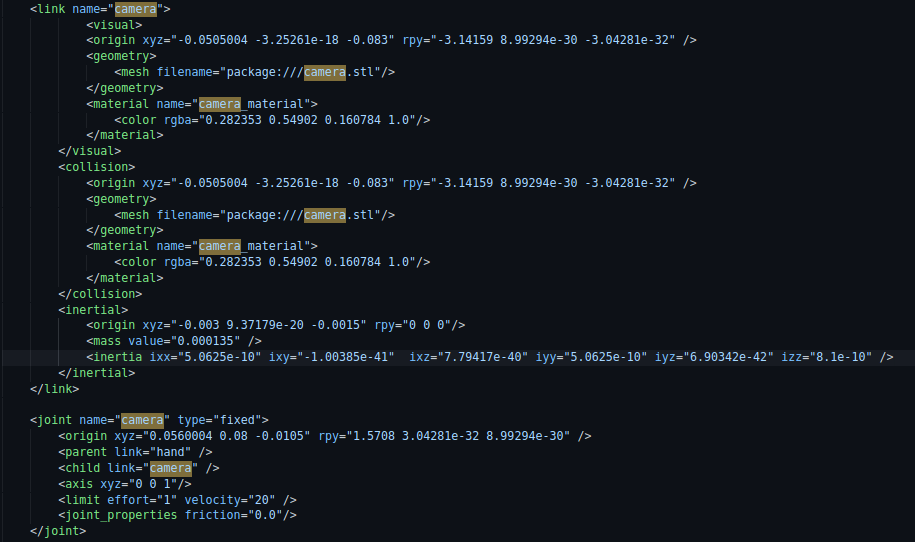
\includegraphics[width=0.8\textwidth]{images/Section04/urdf.png}
    \caption{URDF file extract}
    \label{fig:mesh11}
\end{figure}
\FloatBarrier

\subsection{Forward kinematics}

\hspace{\parindent} To calculate the forward kinematics of our arm we used two different methods. This allowed us to compare the results and validate them. 

\subsubsection{Matlab simulation}

\hspace{\parindent} To begin with, Matlab offers the possibility to import a URDF file describing a robot to make a Simulink model using the simscape toolbox. This is the easiest method when you have the URDF file. It also has the advantage of visually simulating the robot. Indeed, the model is based on the stl files of each part. To create the model, simply run the following command in Matlab : \textbf{smimport(\textit{path to urdf})}

\bigbreak
It will open a simulink file, once it is created, the joints must be modified so that the motor torque is calculated automatically and the desired angles can be entered manually. Finally, a position sensor linking the reference frame and the target frame must be added. We can then obtain the position of the hand for a given angle vector. 

\bigbreak
\begin{figure}[ht]
    \centering
    \includegraphics[width=1\textwidth]{images/Section04/matlab\_robot\_model.png}
    \caption{Simulink model}
    \label{fig:mesh12}
\end{figure}
\FloatBarrier

\bigbreak
\begin{figure}[ht]
    \centering
    \includegraphics[width=0.8\textwidth]{images/Section04/simulink\_model.png}
    \caption{Matlab robot visualization}
    \label{fig:mesh13}
\end{figure}
\FloatBarrier

\bigbreak
It should be noted that a target block positioned at the center of the fingers has been added in the Onshape model. It is in fixed link with the hand and this link is defined in the general assembly. Thus, when creating the URDF file, this target appears separately. It allows to have an easy way to locate it. the mass of this object, which must be defined is $10^{-5}$, to be considered as zero.. The same thing has been done at level of the camera position. 

\subsubsection{Python simulation}

\textbf{Definition :} Let $S = (w,v)$ be a screw axis. If $\|w\|=1$ then, for any distance $\theta\in\mathbb{R}$ traveled along the axis,
\begin{center}
    $e^{[S]\theta}=
    \begin{bmatrix}
        e^{[w]\theta} & (I\theta+(1-\cos\theta)[w]+(\theta-sin\theta)[w]^2)v\\
        0 & 1
    \end{bmatrix}$
\end{center}
If w=0 and $\|v\|=1$ then 
\begin{center}
    $e^{[S]\theta}=\begin{bmatrix}
        I & v\theta\\
        0 & 1
    \end{bmatrix}$
\end{center}

\bigbreak
The second approach is more theoretical and is based on the kinematic parameters seen previously. To realize the calculations we used the python library modern robotics. It has already created functions to calculate the direct kinematics. 

\bigbreak
This library is based on the exponentials of matrices to calculate the position of the end effector from the coordinates of each link. It uses the following formula: 

\begin{center}
    $T(\theta) = e^{[S_1]\theta_1}e^{[S_2]\theta_2}e^{[S_3]\theta_3}e^{[S_4]\theta_4}M$    
\end{center}
where $\theta$ is a $4\times1$ vectors of joint coordinates, $S_i$ is the screw axes of the joint i and M is the transformation matrix when the robot is at its zero configuration.


\bigbreak
So we can use the function FKinSpace which takes as arguments M,$\theta$ and $S_{list}$ as defined above. Depending on whether we want the position of the camera or the end effector, we just have to change the M matrix. This method was faster to perform the calculations and faster to test a large number of values. However, it does not allow visualization.

\begin{minted}[linenos=true,bgcolor=LightYellow]{Python}
# import kinematics parameters
from parameters import * 
import modern_robotics as mr
# define desired angles 
thetalist = np.array([0,0,0,0])
# get transformation matrix and extract the position
t = mr.FKinSpace(m_c,screw_list,thetalist)
p = t.dot(np.array([0,0,0,1]))[:-1]
\end{minted}

\bigbreak
For the same set of angles, we then obtain the following results using Matlab and python: 
\begin{table}[ht]
    \centering
    \begin{tabular}{|p{4cm} | p{4.5cm} | p{4.5cm}|} 
        \hline
        \textbf{joints (rad)} & \textbf{Matlab position (m)} & \textbf{Python Position (m)}\\ [0.3ex] 
        \hline\
        [0 0 0 0] & [-0.4527 0.00063 0.3455] & [-0.4527 0.00063 0.3455] \\ 
        \hline
        [pi/4,-pi/3,0,pi/3] & [-0.1286 0.06948 0.07537] & [-0.1286  0.06949 -0.07533] \\ 
        \hline
        [pi/4,pi/6,-pi/6,pi/3]& [-0.2259 0.1668 0.4583] & [-0.2258  0.1667  0.4583] \\ 
        \hline
    \end{tabular}
    \caption{Matlab and Python result for forward kinematics}
\end{table}

\bigbreak
As we can see, the results are identical at $10^{-4}m$. We can therefore validate the kinematic model of our robot. The position of matlab is correct since it comes from an explicit model and allows a visualization.

\subsection{Inverse kinematics}

\hspace{\parindent} In the same way we used two methods to calculate the inverse kinematics. The objective is to determine the coordinates of each link from a given position.

\subsubsection{Matlab simulation}

\hspace{\parindent} Once we had a simulink model, we were able to create a matlab variable that represents the robot. It is obtained with the script below.  This variable contains information about each link (position, parent, child) but also about each body (mass, center of mass and inertia). The bodies are numbered from 1 to 7. The number 1 corresponds to the base and 7 to the end effector. We could identify them from the information on the mass and inertia.

\begin{minted}[linenos=true,bgcolor=matlabColor]{matlab}
%% create robot matrix
open_system('robot.slx')
S=sim('robot.slx')
[robot,importInfo] = importrobot(gcs)
robot.DataFormat = 'column';
\end{minted}

\bigbreak
The Robotic System toolbox then allows to calculate the inverse kinematics. Indeed, there is a block \textit{inverse kinematics} which takes as input a desired configuration (transformation matrix), weights which allow to adjust the importance of reaching the desired rotation and translation according to the 3 axes and returns the list of the coordinates of each link. This block takes as parameter the robot variable created before. You must then indicate the name of the body corresponding to the end effector. 

\bigbreak
The block also offers the possibility to choose the resolution method. We have selected the Levenber-Marquardt method leaving the original resolution parameters. This method requires to provide an initial value, if possible close to the real value. As we will explain in the following parts, our robot will always start in the same position. We therefore provided this angle vector as origin.

\bigbreak
\begin{figure}[ht]
    \centering
    \includegraphics[width=0.8\textwidth]{images/Section04/inverse\_kinematics\_matlab.png}
    \caption{Inverse kinematics simulink}
    \label{fig:mesh14}
\end{figure}
\FloatBarrier

\bigbreak
We are only interested in the position of the hand. Indeed, the hand being symmetrical the orientation of the fingers to catch objects is not important. Thus, the points for the orention are null and the points for the position are at the maximum.

\bigbreak
To verify the validity of the method, we retrieved the values of the link coordinates found by this block for desired end effector positions. Then, we submitted the robot in direct kinematics to this angles and verified that the positions are the same. Even if we know a set of angles corresponding to this position, depending on the initial hypothesis, the angles found can be different. Thus, comparing the value of the angles is not a good way to make sure that the resolution is working properly. As we do not take into account the orientation, we have only compared the positions.

\begin{table}[ht]
    \centering
    \begin{tabular}{|p{4.5cm} | p{4.5cm} | p{5cm}|} 
        \hline
        \textbf{desired position (m)} & \textbf{real position (m)} & \textbf{angles (rad)}\\ [0.3ex] 
        \hline\
        [-0.4527 0.00063 0.3455] & [-0.4542 0.00063 0.3455] & [$9.10^{-6}$ $9.10^{-3}$ $9.10^{-3}$ 0] \\ 
        \hline
        [-0.1286 0.06948 0.07537] & [-0.1288 0.06968 0.0739] & [0.7854  0.6981 0.7006 1.377] \\ 
        \hline
        [-0.2259 0.1668 0.4583] & [-0.2269 0.1678 0.4585] & [0.7855  0.6981  -0.1312 0.6766] \\ 
        \hline
    \end{tabular}
    \caption{Inverse kinematics results with Matlab}
\end{table}
\FloatBarrier

\bigbreak
In the case of the table above, the initial assumption is always [0 0 0 0]. The desired position and the actual position are identical at $10^{-3}m$. We can therefore validate the model. Nevertheless, the closer the initial value is to the final result, the smaller the error is. As we will see later, in our case, the arm will start in its zero configuration. We therefore know the value of these angles. In order to be as accurate as possible, this will be our starting point for calculating the inverse kinematics in all cases. As we can see from the table, this is sufficient to obtain a satisfactory result in all cases.

\subsubsection{Python simulation}

\subsubsection{Torque Study}
\subsubsection{General principal}

\subsubsection{Joint results}

\subsubsection{Hardware choices}
